%% start of file `template.tex'.
%% Copyright 2006-2015 Xavier Danaux (xdanaux@gmail.com).
%
% This work may be distributed and/or modified under the
% conditions of the LaTeX Project Public License version 1.3c,
% available at http://www.latex-project.org/lppl/.


\documentclass[11pt,a4paper,sans]{moderncv}        % possible options include font size ('10pt', '11pt' and '12pt'), paper size ('a4paper', 'letterpaper', 'a5paper', 'legalpaper', 'executivepaper' and 'landscape') and font family ('sans' and 'roman')
\usepackage{ragged2e}
\usepackage{lastpage}

\usepackage{fancyhdr}
\usepackage{pdfpages}
\fancyfoot[C]{ \thepage\ / \pageref{LastPage}}

% moderncv themes
\moderncvstyle{classic}                             % style options are 'casual' (default), 'classic', 'banking', 'oldstyle' and 'fancy'
\moderncvcolor{blue}                               % color options 'black', 'blue' (default), 'burgundy', 'green', 'grey', 'orange', 'purple' and 'red'
%\renewcommand{\familydefault}{\sfdefault}         % to set the default font; use '\sfdefault' for the default sans serif font, '\rmdefault' for the default roman one, or any tex font name
%\nopagenumbers{}                                  % uncomment to suppress automatic page numbering for CVs longer than one page

% character encoding
%\usepackage[utf8]{inputenc}                       % if you are not using xelatex ou lualatex, replace by the encoding you are using
%\usepackage{CJKutf8}                              % if you need to use CJK to typeset your resume in Chinese, Japanese or Korean

% adjust the page margins
\usepackage[scale=0.75]{geometry}
%\setlength{\hintscolumnwidth}{3cm}                % if you want to change the width of the column with the dates
%\setlength{\makecvtitlenamewidth}{10cm}           % for the 'classic' style, if you want to force the width allocated to your name and avoid line breaks. be careful though, the length is normally calculated to avoid any overlap with your personal info; use this at your own typographical risks...

% personal data
\name{Fabian E.}{Gruber}
%\title{Resumé title}                               % optional, remove / comment the line if not wanted
\address{Anna-Stainer-Knittel-Weg 3/5/4}{6020 Innsbruck, Austria}% optional, remove / comment the line if not wanted; the "postcode city" and "country" arguments can be omitted or provided empty
\phone[mobile]{+43~650~2587521}                   % optional, remove / comment the line if not wanted; the optional "type" of the phone can be "mobile" (default), "fixed" or "fax"
%\phone[fixed]{+2~(345)~678~901}
%\phone[fax]{+3~(456)~789~012}
\email{Fabian.Gruber@uibk.ac.at}                               % optional, remove / comment the line if not wanted
%\homepage{www.johndoe.com}                         % optional, remove / comment the line if not wanted
%\social[linkedin]{john.doe}                        % optional, remove / comment the line if not wanted
%\social[twitter]{jdoe}                             % optional, remove / comment the line if not wanted
%\social[github]{jdoe}                              % optional, remove / comment the line if not wanted
%\extrainfo{additional information}                 % optional, remove / comment the line if not wanted
\photo[64pt][0.4pt]{IMG_3890_cropped2}                       % optional, remove / comment the line if not wanted; '64pt' is the height the picture must be resized to, 0.4pt is the thickness of the frame around it (put it to 0pt for no frame) and 'picture' is the name of the picture file
%\quote{}                                 % optional, remove / comment the line if not wanted

% bibliography adjustements (only useful if you make citations in your resume, or print a list of publications using BibTeX)
%   to show numerical labels in the bibliography (default is to show no labels)
\makeatletter\renewcommand*{\bibliographyitemlabel}{\@biblabel{\arabic{enumiv}}}\makeatother
%   to redefine the bibliography heading string ("Publications")
%\renewcommand{\refname}{Articles}

% bibliography with mutiple entries
%\usepackage{multibib}
%\newcites{book,misc}{{Books},{Others}}
%----------------------------------------------------------------------------------
%            content
%----------------------------------------------------------------------------------
\begin{document}
%\begin{CJK*}{UTF8}{gbsn}                          % to typeset your resume in Chinese using CJK

%-----       letter       ---------------------------------------------------------
% recipient data
\recipient{Airborne Technologies GmbH \\z.H. Teresa Mancevski}{Viktor Lang Stra{\ss}e 8\\A-2700 Wiener Neustadt}
\date{22. Nov, 2018}
\opening{Sehr geehrte Frau Mancevski,}
\closing{Mit besten Gr\"{u}{\ss}en,}
\enclosure[Anhang]{Lebenslauf, Publikationsliste und Diplombescheid}  % use an optional argument to use a string other than "Enclosure", or redefine \enclname

\makelettertitle
\justify
Ich m\"{o}chte mich hiermit f\"{u}r die Stelle 'Mitarbeiter in der Datenverarbeitung' bewerben. Zur Zeit bin ich als wissenschaflicher Mitarbeiter am Institut f\"{u}r Geographie der LFU Innsbruck angestellt, wo ich auch an meiner Dissertation mit dem Arbeitstitel "Digital terrain analysis to support soil survey" arbeite.

Die intensive Besch\"{a}ftigung mit Photogrammetrie und Fernerkundung begann wahrend  meines Studiums der Kulturtechnik und Wasserwirtschaft an der Universit\"{a}t f\"{u}r Bodenkultur in Wien. Neben den Lehrveranstaltungen und \"{U}bungen der Grundlagenf\"{a}cher Vermessungswesen sowie Photogrammetrie und Fernerkundung absolvierte ich auch den vertiefenden Wahlfachblock Photogrammetrie und Fernerkundung, welcher neben der Angewandten Geologie das zweite Pr\"{u}fungsfach meiner Diplompr\"{u}fung war. Als studentischer Mitarbeiter am Institut f\"{u}r Angewandte Geologie sammelte ich erste praktische Erfahrung in der Bearbeitung und Analyse von Fernerkundungsdaten. Im konkreten Projekt 'Remote Geohazards Assessment in Tajikistan (TajHaz)' besch\"{a}ftigte ich mich neben der Digitalisierung von Wasserfl\"achen und Gletschergebieten auch mit der \"uberwachten Klassifizierung dieser Fl\"achen anhand von Landsat und ASTER Satellitendaten.  Die gr\"undliche Besch\"aftigung und Erfahrung in der Arbeit mit Geoinformationssystemen erschloss mir auch die M\"oglichkeit noch w\"ahrend des Studiums als Tutor f\"{u}r die \"{U}bung "Einf\"uhrung in GIS" zu arbeiten sowie nach dem Abschluss meines Studiums in einem Nachfolgeprojekt am Institut f\"{u}r Angewandte Geologie angestellt zu werden. Hierbei verst\"arkte sich die Anwendung von freien Geoinformationsystemen wie etwa GRASS GIS, unter anderem f\"{u}r die Landbedeckungskartierung in schwer zug\"anglichen Gebieten in Tajikistan anhand von Satellitenfernerkundung und digitalen Gel\"andemodellen. Weiters erhielt ich erste Einblicke in die Anwendung von Radarfernerkundung zur Kartierung von Massenbewegungen mit der Software Sarscape, welche ich vor Kurzem durch den Abschluss des Onlinekurses "Echoes in Space - Introduction to radar remote sensing' der European Space Agency mit der Anwendung des frei verf\"ugbaren Tools 'SNAP' vertieft habe.

Nach dem Wechsel an die LFU Innsbruck, wo ich eine Stelle als Projektmitarbeiter am Institut f\"{u}r Geographie mit M\"{o}glichkeit der Verfassung einer Dissertation antrat, begann die intensivierte Besch\"{a}ftiung mit digitalen Gel\"andemodellen. In meiner T\"{a}tigkeit im Rahmen mehrerer Projekte analysiere ich die Anwendbarkeit des aus ALS-Daten entstandenen, und vom Land S\"udtirol zur Verf\"{u}gung gestellten, DGMs f\"ur Boden- sowie Blaikenkartierungen. In einer Publikation verglich ich etwa die Ergebnisse verschiedener automatisierter Gel\"{a}ndeklassifikationsalgorithmen hinsichtlich derer Eignung, das Gel\"{a}nde im Sinne des Bodenkartierers, und dessen Boden-Landschaft-Modells, einzuteilen. Weiters untersuchte ich inwieweit aus DGMs abgeleitete Gel\"{a}ndeparameter imstande sind, geologische Einheiten zu charakterisieren, etwa hinsichtlich Oberfl\"{a}chenrauhigkeit. F\"{u}r die genannten Analysen und \"{a}hnliche Aufgaben im Rahmen weiterer Projekte greife ich gerne auf Methoden aus dem Bereich des maschinellen Lernens bzw. der statistischen Modellierung zur\"{u}ck. Hierf\"{u}r verwende ich R, eine freie Programmiersprache f\"{u}r statistisches Rechnen, sowie die freien Geoinformationssysteme  GRASS und SAGA, sowie QGIS zur Visualisierung der Ergebnisse. Neben der Prammiersprache R  verwende ich auch Python Scripts zur Automatisierung von Workflows.

Aufgrund meiner langj\"{a}hrigen Erfahrung als Projektmitarbeiter an verschiedenen Universit\"{a}ten bringe ich viel Erfahrung in selbstst\"{a}ndiger Arbeit mit. Weiters bringe ich die F\"{a}higkeit mich rasch in neue Themen einzuarbeiten sowie ein ausgepr\"{a}gtes Interesse an Fernerkundungsmethoden und deren Verwendung in verschiedensten Anwendungsgebieten. Ein Blick auf die auf der Homepage angef\"{u}hrten vergangenen Projekte ihrer Firma hat daher mein Interesse geweckt. Da ich potentiell noch ein Jahr in Innsbruck verbringen werde, danach aber eine R\"uckkehr nach Wien oder Umgebung anstrebe, interessiere ich mich vorerst f\"{u}r die Stelle as Mitarbeiter in der Datenverarbeitung sowie die M\"{o}glichkeit von Homeoffice sowie Teilzeit, da ich bei einem Wochenstundenausma{\ss} von etwa 25 Stunden weiter an meiner Dissertation und deren Abschluss arbeiten k\"onnte. 

\"{U}ber eine Einladung zu einem Gespr\"ach w\"urde ich mich freuen.

\makeletterclosing
\clearpage
%-----       resume       ---------------------------------------------------------
\makecvtitle


\section{Berufserfahrung}
\cventry{2013--Heute   }{Wissenschaftlicher Mitarbeiter}{Institut f\"{u}r Geographie, Universit\"{a}t Innsbruck}{Innsbruck}{}{Forschungsprojekte: 
\begin{itemize}%
\item Shallow erosion dynamics in mountain grasslands of South Tyrol: Monitoring, process analysis and mitigation measures (EroDyn)
  \begin{itemize}%
  \item Geodatenmanagement 
   \item Gel\"{a}ndeklassifizierung f\"{u}r automatisierte Blaikenkartierung
   \item Dispositionskartierung auf Landesebene
   \end{itemize}
\item ReBo -- Reliefklassifizierung aus ALS Daten als Grundlage f\"ur die Regionalisierung von Bodendaten
  \begin{itemize}%
  \item Ableitung von Landschaftseinheiten mit maschinellem Lernen und automatisierten Gel\"{a}ndeklassifikationsalgorithmen
  \item Bodenkundliche Feldarbeit
  \item Mitarbeit bei der Entwicklung der Java-Applikation "SEPP" (Soil Evaluation in Planning Procedures) f\"{u}r Bodenfunktionsbewertungen
  \end{itemize}
\end{itemize}}
\cventry{2016--2017}{Universit\"{a}tsdozent}{Institut f\"{u}r Geographie, Universit\"{a}t Innsbruck}{Innsbruck}{}{\"{U}bungen zur Statistik mit R (2 Semester)}
\cventry{2016--2017}{Bildungskarenz}{}{}{}{Arbeit an Dissertation mit dem Arbeitstitel 'Digital terrain analysis to support field soil survey'}
\cventry{2011--2013}{Wissenschaftlicher Mitarbeiter}{Institut f\"{u}r Angewandte Geologie, BOKU}{Wien}{}{Forschungsprojekte: 
\begin{itemize}%
\item Hazard assessment for an expected dam break flood in the Hunza Valley, Pakistan: A combination of GIS, Remote Sensing, and computer simulation techniques
\begin{itemize}%
  \item Dammbruch-Modellierung mit BREACH
  \item Hydraulische Modellierung mit FLO-2D
  \end{itemize}
\item Poverty Alleviation through Mitigation of Integrated High-Mountain Risk (PAMIR)
\begin{itemize}%
  \item Kartierung von Naturgefahren, Gletschern und Infrastruktur mit GIS und Fernerkundungsmethoden
  \end{itemize}
  \end{itemize}}
\cventry{2009--2010}{Projektmitarbeiter}{Institut f\"{u}r Angewandte Geologie, BOKU}{Wien}{}{Forschungsprojekt: 
\begin{itemize}%
\item Remote Geohazards Assessment in Tajikistan (TajHaz)
\begin{itemize}%
  \item Kartierung von Naturgefahren und Gletscherseen anhand von Satellitenbildern  und GIS
  \item Feldarbeit in Tajikistan
  \end{itemize}
  \end{itemize}}

\cventry{2010--2011}{Tutor}{ Institut f\"ur Landschaftsentwicklung, Erholungs- und Naturschutzplanung, BOKU }{Wien}{}{Tutor f\"ur ArcGIS im Rahmen der LV "Einf\"uhrung in GIS"}

\section{Ausbildung}
\cvitem{2002--2011}{Diplomstudium der Kulturtechnik und Wasserwirtschaft an der Universit\"{a}t f\"{u}r Bodenkultur (BOKU), Wien}
\cvitem{1993--2001}{Linz International School Auhof, Linz:
Abschluss mit Matura und International Baccalaureate (IB)}
\cvitem{1991--1993}{Volksschule Linz-Pichling}
\cvitem{1989--1991}{Lincoln Elementary School Pittsburgh, PA, USA}

\section{Diplomarbeit}
\cvitem{title}{\emph{The 2010 Attabad Landslide Dam Lake:
modeling and prediction of Lake Outburst
Floods}}
\cvitem{Betreuer}{Jean F. Schneider and Martin Mergili}

\section{Sprachen}
\cvitemwithcomment{Deutsch}{Muttersprache}{ }
\cvitemwithcomment{Englisch}{Verhandlungssicher}{ }
\cvitemwithcomment{Spanisch}{Grundkenntnisse}{ }
\cvitemwithcomment{Franz\"osisch}{Grundkenntnisse}{ }

\section{EDV-Kenntnisse}
\cvdoubleitem{Operating systems}{Linux (Ubuntu), Windows} {Languages}{R, Python, Bash}
\cvdoubleitem{Geographic information systems}{ArcGIS, GRASS, SAGA, QGIS } {Text- verarbeitung } {MS Word, Libreoffice,  \LaTeX{} with Texmaker}
\cvdoubleitem{Bild- verarbeitung}{GIMP, Inkscape} {Modellierungs- software } {FLO-2D, Ramms, Dan-3D}
\section{Hobbies}
\cvitem{G\"artnerei}{Mitarbeit beim Gemeinschaftsgarten der Vinzigemeinschaft Waldhuttl, Innsbruck}
\cvitem{Reisen}{Reisen durch Mittel und S\"udamerika, Zentralasien, S\"udostasien und Madagaskar}

% Publications from a BibTeX file without multibib
%  for numerical labels: \renewcommand{\bibliographyitemlabel}{\@biblabel{\arabic{enumiv}}}% CONSIDER MERGING WITH PREAMBLE PART
%  to redefine the heading string ("Publications"): 
\renewcommand{\refname}{Publikationen}
\nocite{*}
\bibliographystyle{plain}
\bibliography{publications3}   
\section{Publikationen}
\subsection{Peer-reviewed journal articles and book chapters}
\cvitem{[1]}{Gruber, F.E., Baruck, J., Geitner, C. (2017):  Algorithms vs. surveyors: a comparison of automated landform delineations and surveyed topographic positions from soil mapping in an Alpine environment. Geoderma 308, 9-25.}
\cvitem{[2]}{Geitner, C., Baruck, J., Freppaz, M., Godone, D., Grashey-Jansen, S., Gruber, F.E., Heinrich, K., Papritz, A., Simon, A., Stanchi, S., Traidl, R., von Albertini, N., Vrscaj, B. (2017). Soil and land use in the Alps -- Challenges and examples of soil survey and soil data use to support sustainable development. In: Pereira, P., Brevik, E.C., Munoz-Rojas, M., Miller, B. (Eds.), Soil mapping and process modelling for sustainable land use management. Elsevier, Amsterdam. 221-292}
\cvitem{[3]}{Baruck, J., Nestroy, O., Sartori, G., Baize, D., Traidl, R., Vrisaj, B., Br{\"a}m, E., Gruber, F.E., Heinrich, K., Geitner, C. (2016): Soil classification
and mapping in the Alps: The current state and future challenges .
Geoderma 264, Part B, 312--331.}
\cvitem{[4]}{Zieher, T., Gruber, F.E.; Rutzinger, M.; Mei{\ss}l, G.; Geitner, C.; Perzl, F. (2016): Data
requirements for the assessment of shallow landslide susceptibility using logistic regression. In: Proceedings of the 12th International Symposium on Landslides - Landslides and Engineered Slopes. Experience, Theory and Practice. Napoli, Italy. CRC Press, S. 2139-2146.}
\cvitem{[5]} {Gruber, F.E., Mergili, M. (2013): Regional-scale analysis of high-mountain multi-hazard and risk indicators in the Pamir (Tajikistan) with GRASS GIS. Natural Hazards and Earth System Sciences 13: 2779-2796.}
\cvitem{[6]} {Schneider, J.F., Gruber, F., Mergili, M. (2013): Impact of large landslides, mitigation measures. In: Genevois, R., Prestininzi, A. (eds.): International Conference on Vajont - 1963-2013 - Thoughts and analyses after 50 years since the catastrophic landslide. Proceedings of the International Conference Vajont 1963-2013, Padua, Italy, October 8-10, 2013. Italian Journal of Engineering Geology and Environment - Book: 73-84.}
\cvitem{[7]} {Schneider, J.F., Gruber, F.E., Mergili, M. (2013): Recent Cases and Geomorphic Evidence of Landslide-Dammed Lakes and Related Hazards in the Mountains of Central Asia. In: Margottini, C., Canuti, P., Sassa, K. (eds.): Landslide Science and Practice: Volume 6: Risk Assessment, Management and Mitigation (Proceedings of the 2nd World Landslide Forum, FAO Headquarters Rome, Italy, October 3-9, 2011): 57-64. Springer, Heidelberg, Berlin, New York}
\subsection{Selected conference abstracts and presentations}
\cvitem{[8]}{Gruber, F.E., Baruck, J. und C. Geitner (2016): Joint analysis of parent material and topography to support soil survey -- a case study from South Tyrol. -- Jahrestagung
der {\"O}sterreichischen Forschungsgruppe f{\"u}r Geomorphologie und Umweltwandel und der Schweizerischen Gesellschaft f{\"u}r Geomorphologie 2016, Innsbruck (23.09.2016).}
\cvitem{[9]}{Gruber F.E., Baruck, J., Simon, A. und C. Geitner (2015): Reliefklassifizierung f{\"u}r die
Erstellung von Bodenkarten anhand von geomorphons (GRASS GIS).--  Posterausstellung im Rahmen der Jahrestagung der Deutschen Bodenkundlichen Gesellschaft, M{\"u}nchen 2015, AG Digital Soil Mapping (09.09.2015). }
\cvitem{[10]}{Gruber, F., Zieher, T., Rutzinger, M. und C. Geitner (2015): Geomorphons and structure metrics for the characterization of geomorphological landscape regions in Austria. EGU General Assembly 2015 (EGU 2015), Wien
(16.04.2015).  }
\cvitem{[11]}{Gruber, F.E., Baruck, J., Rutzinger, M. and C. Geitner (2014): Landform segmentation for
digital soil mapping. -- EGU General Assembly 2014 (28.04.-02.05.2014, Vienna (Austria)), Geophysical Research Abstracts Vol. 16, EGU2014-5644.  }
                   % 'publications' is the name of a BibTeX file

% Publications from a BibTeX file using the multibib package
%\section{Publications}
%\nocitebook{book1,book2}
%\bibliographystylebook{plain}
%\bibliographybook{publications}                   % 'publications' is the name of a BibTeX file
%\nocitemisc{misc1,misc2,misc3}
%\bibliographystylemisc{plain}
%\bibliographymisc{publications}                   % 'publications' is the name of a BibTeX file

\clearpage
%\clearpage\end{CJK*}                              % if you are typesetting your resume in Chinese using CJK; the \clearpage is required for fancyhdr to work correctly with CJK, though it kills the page numbering by making \lastpage undefined
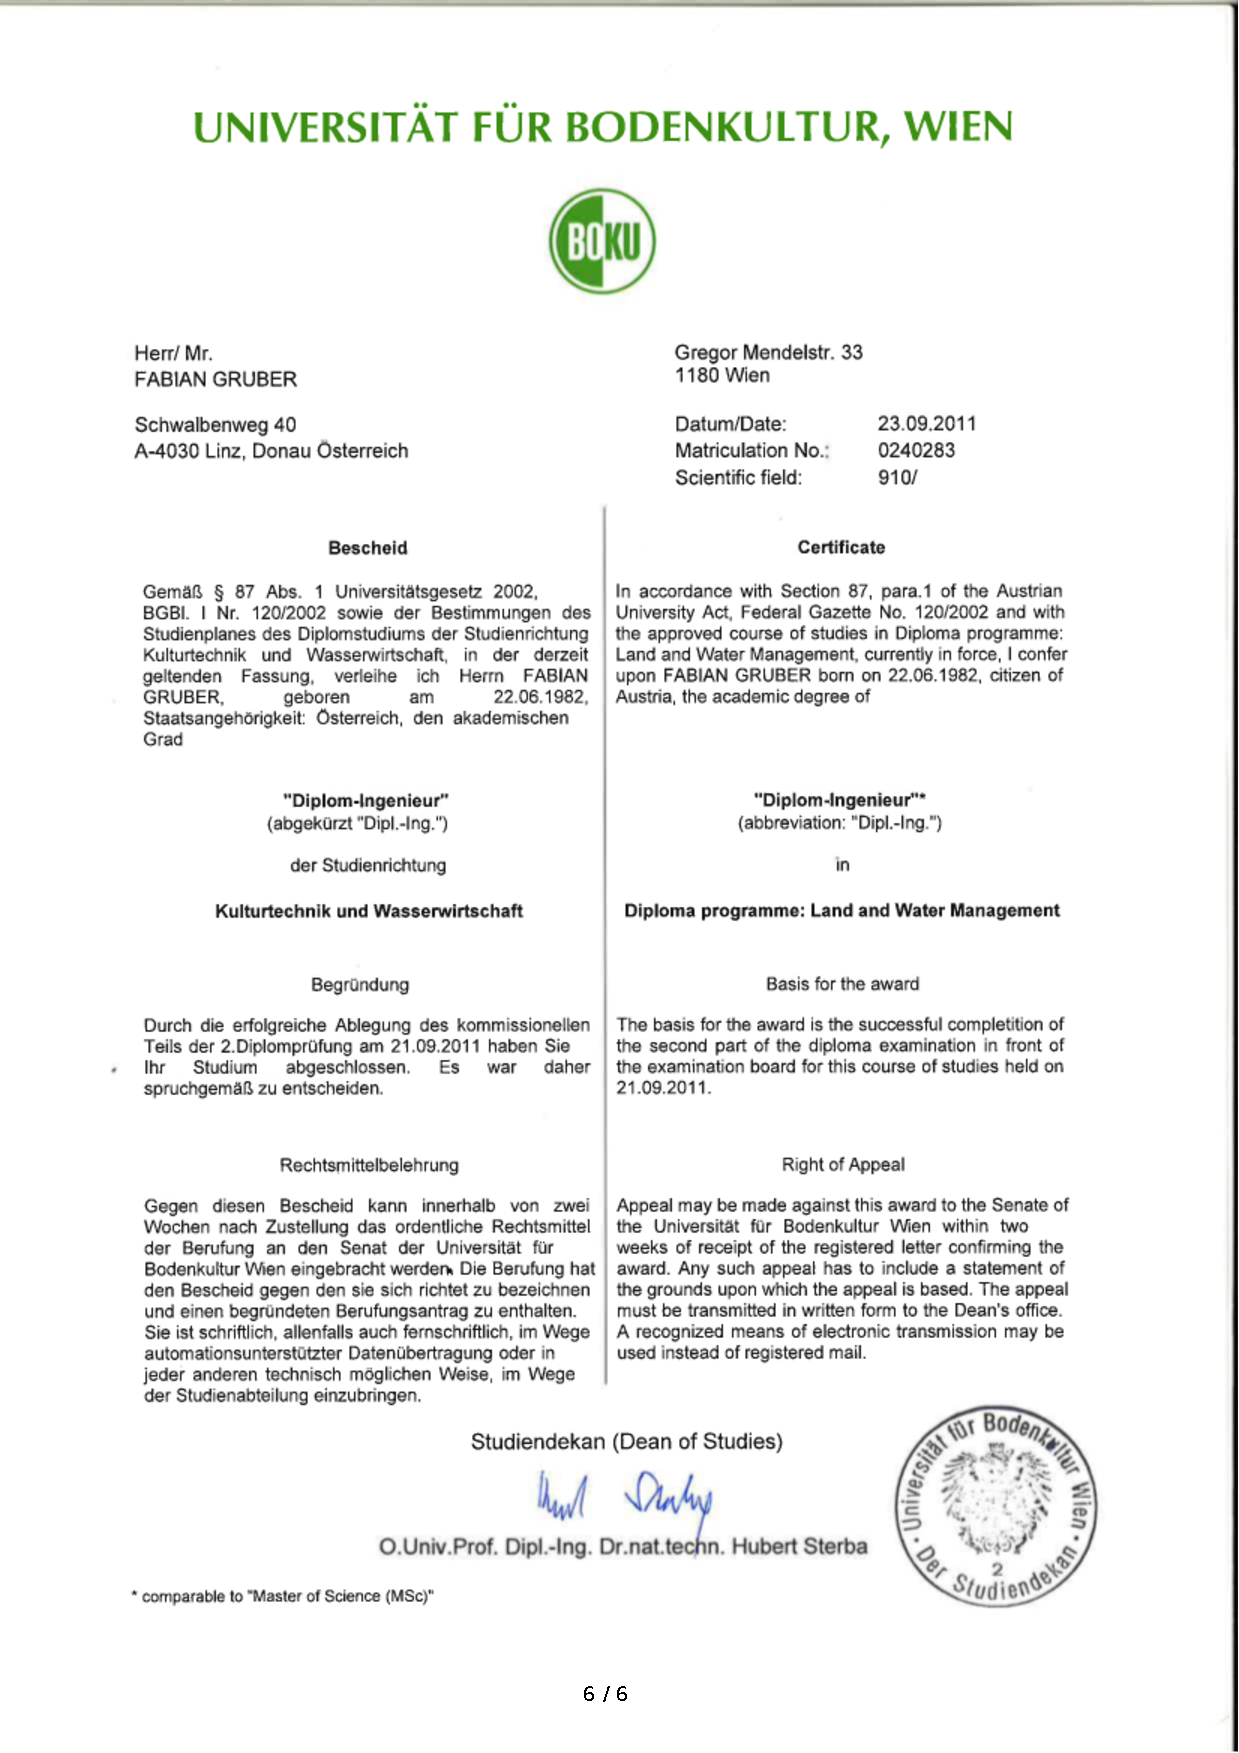
\includepdf{Dipling_seite6von6.pdf}
\end{document}


%% end of file `template.tex'.
